% ICEIC 2027 draft. A4, two columns, 10 pt (ICEIC: 2-6 pages, single-spaced, two-column A4, >= 10 pt).
% Paste the body into the official ICEIC LaTeX template if its preamble differs from IEEEtran.
% Lines marked TODO need the authors' input or a check before submission.
\documentclass[conference,a4paper]{IEEEtran}
\IEEEoverridecommandlockouts
\usepackage{cite}
\usepackage{amsmath,amssymb}
\usepackage{graphicx}
\usepackage{booktabs}
\usepackage{multirow}
\usepackage{xcolor}
\usepackage{tikz}
\usetikzlibrary{positioning,arrows.meta,fit}
\usepackage{pgfplots}
\pgfplotsset{compat=1.18}
\usepgfplotslibrary{groupplots}

\begin{document}

\title{XAD-TTS: Cross-Variety Initialization and Alignment-Supervised Durations for One-Hour Hakka Speech Synthesis}

% TODO: authors and affiliations
\author{\IEEEauthorblockN{Author Name}
\IEEEauthorblockA{Department, University\\
City, Taiwan\\
email@example.edu}}

\maketitle

\begin{abstract}
Hakka is a tonal language with several regional varieties, and recorded speech for most of them is scarce. We study neural text-to-speech (TTS) for two Taiwanese Hakka varieties, Sixian and Hailu, when only one hour of target-variety speech is available. With so little data, a TTS model that learns its own alignment produces imprecise segment timing and weak tones. We present XAD-TTS, a training recipe for Matcha-TTS that initializes the model from a sibling variety and supervises an enlarged duration predictor with forced-alignment durations. Across three training seeds, XAD-TTS raises the share of checked-syllable vowels whose duration, measured on the synthesized waveform, lies within $\pm$30\,ms of natural speech from 71.0\% to 81.3\% (Sixian) and from 69.4\% to 82.2\% (Hailu), on par with a baseline trained on about 48 times more data. It also lowers mel-cepstral distortion by 0.33 and 0.24\,dB and raises objective tone recognition by 8.8 and 5.3 points. An independent check with a multilingual speech recognizer confirms that checked syllables and tone marks are better preserved.
\end{abstract}

\begin{IEEEkeywords}
speech synthesis, low-resource languages, Hakka, transfer learning, duration modeling, forced alignment
\end{IEEEkeywords}

\section{Introduction}

Hakka is a Sinitic tonal language. In Taiwan it is spoken in several regional varieties, two of the major ones being Sixian and Hailu. The two share most consonants and vowels but differ in their tone systems. Speech technology for Hakka has begun to appear~\cite{chen2024voxhakka}, yet the recorded speech available for each variety is limited, and a voice for a new variety or speaker often has to be built from very little data.

Neural TTS models such as Matcha-TTS~\cite{mehta2024matcha} learn the alignment between input symbols and acoustic frames during training, typically with monotonic alignment search (MAS)~\cite{kim2020glow}, and train a duration predictor on the resulting durations. With one hour of data, both the learned alignment and the predictor are noisy. In Hakka this affects more than naturalness: checked syllables, the syllables of the entering tones that end in an unreleased stop (written \textit{-b}, \textit{-d}, \textit{-g}), are marked by a short vowel, so segment timing carries a phonological contrast.

Two ideas have been used separately for low-resource TTS: initializing from a model of a related, better-resourced language~\cite{chen2019crosslingual,xu2020lrspeech}, and replacing learned alignments with durations from an external aligner, as FastSpeech~2~\cite{ren2021fastspeech2} does with the Montreal Forced Aligner (MFA)~\cite{mcauliffe2017mfa}. We combine both for Hakka and ask how far one hour of target-variety data can go. Our contributions are:
\begin{itemize}
\item \textbf{XAD-TTS}, a training recipe that initializes from a sibling variety and supervises an enlarged duration predictor with forced-alignment durations. The aligner is needed only for training; no component is added at inference.
\item Controlled experiments on two varieties, three data sizes (1, 10, and about 48\,h), and three training seeds, with segment timing measured on the synthesized waveforms.
\item An evaluation that goes beyond spectral distance: objective tone recognition and an independent check with a multilingual speech recognizer.
\end{itemize}

\section{Method}

\subsection{Base model}
Matcha-TTS~\cite{mehta2024matcha} encodes the input symbols into per-symbol features and log-durations, upsamples the features by the durations, and generates a mel spectrogram with a conditional flow-matching decoder~\cite{lipman2023flow}; a HiFi-GAN vocoder~\cite{kong2020hifigan} produces the waveform. During training, MAS chooses the durations that best explain the mel frames under the encoder output, and the duration predictor is fitted to them. The training loss is the sum of the duration, prior, and flow-matching losses. At inference, predicted durations are rounded up to whole frames.

\subsection{Cross-variety initialization}
The source model is trained from scratch on the full training pool of the other variety (48.0\,h for Sixian, 47.2\,h for Hailu). Both varieties use one symbol table, so every target parameter with a matching name and shape is copied from the source. Speaker embeddings are re-initialized, nothing is frozen, and the optimizer starts afresh at step 0. The copied mel normalization statistics belong to the source variety, so synthesis always uses the statistics of the target training data.

\subsection{Alignment-supervised durations}
We trained an MFA acoustic model and a pronunciation lexicon on the corpus and aligned every training utterance. Phone intervals are converted to frame counts (hop 256 at 22.05\,kHz, i.e., 11.6\,ms per frame). Matcha-TTS inserts a blank token between symbols; aligned pauses are assigned to the corresponding blank, and every blank receives at least one frame, taken from the preceding phone. These durations replace MAS: they are the targets of the duration loss and define the upsampling used by the prior and decoder losses.

\subsection{Larger duration predictor and rounding}
To give the duration predictor more capacity, we enlarge it from kernel size 3 and 256 channels to kernel size 5 and 512 channels. With cross-variety initialization, the enlarged predictor and the speaker embeddings are the only re-initialized parts. Rounding every predicted duration up adds about half a frame per symbol on average, which can lengthen segments when the predictor itself is unbiased. We therefore choose, for every trained model, between rounding up and cumulative rounding (rounding the running sum, which preserves the total length): the rule whose vowel durations on the validation set are closer to the training targets is used. The same selection procedure is applied to all systems, including the baseline.

XAD-TTS combines Sections~II-B to II-D. Figure~\ref{fig:overview} summarizes the recipe and the evaluation.

\begin{figure}[t]
\centering
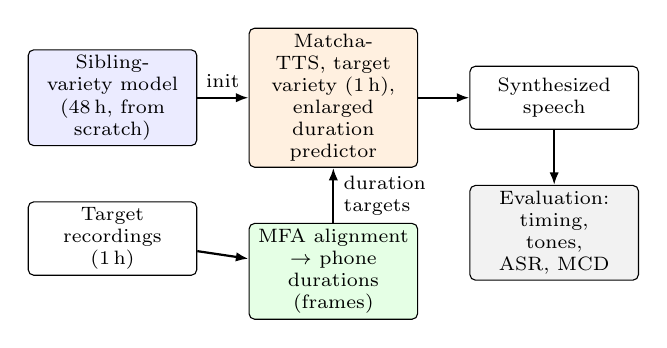
\begin{tikzpicture}[
  font=\scriptsize, node distance=7mm and 6.5mm,
  box/.style={draw, rounded corners=2pt, align=center, minimum height=8mm, text width=20mm, inner sep=2pt, fill=#1},
  box/.default=white, arr/.style={-{Latex[length=1.6mm]}, thick}]
\node[box=blue!8] (src) {Sibling-variety model\\(48\,h, from scratch)};
\node[box=orange!12, right=of src] (tts) {Matcha-TTS, target\\variety (1\,h), enlarged\\duration predictor};
\node[box, right=of tts] (syn) {Synthesized\\speech};
\node[box, below=of src] (wav) {Target recordings\\(1\,h)};
\node[box=green!10, below=of tts] (mfa) {MFA alignment\\$\rightarrow$ phone durations\\(frames)};
\node[box=gray!10, below=of syn] (eval) {Evaluation: timing,\\tones, ASR, MCD};
\draw[arr] (src) -- node[above]{init} (tts);
\draw[arr] (tts) -- (syn);
\draw[arr] (wav) -- (mfa);
\draw[arr] (mfa) -- node[right, align=left]{duration\\targets} (tts);
\draw[arr] (syn) -- (eval);
\end{tikzpicture}
\caption{XAD-TTS: the target model starts from a sibling-variety model, and its enlarged duration predictor is trained on forced-alignment durations instead of self-learned alignments.}
\label{fig:overview}
\end{figure}

\section{Experimental Setup}

\subsection{Data}
We use the TTS part of the Hakka Across Taiwan (HAT) corpus~\cite{hat2024}: read speech in Sixian and Hailu, each by one professional female and one professional male speaker. Validation and test sets are defined by recording prompt, so their prompts never occur in training. Training subsets of 1\,h and 10\,h are balanced across the two speakers and nested (the 10\,h set contains the 1\,h set). Pinyin is split deterministically into initial, vowel nucleus, and coda, and the tone is attached to the nucleus symbol (``joint'' symbols); Section~IV-A also uses ``separate'' symbols, in which tones are separate inputs, so 84\% instead of 55\% of the symbols are shared by the two varieties. Over 99\% of the utterances were aligned successfully.

\subsection{Systems and training}
We compare \textbf{Base} (scratch, MAS), \textbf{+AD} (scratch, alignment-supervised durations), and \textbf{XAD} (cross-variety initialization, alignment-supervised durations, enlarged predictor), all with joint symbols. Each is trained with Adam (learning rate $10^{-4}$, batch 16) for a fixed 40{,}000 steps with three training seeds (1234, 123, 2026) at 1\,h and 10\,h; the 40{,}000-step checkpoint is evaluated. As a high-resource reference, a Base model is trained on the full pool (48.0\,h / 47.2\,h) with early stopping (single seed). One 40{,}000-step run takes about 2\,h on a single RTX~5070~Ti GPU (about 5.3 steps/s, 3.9\,GB memory); the Base model has 20.9\,M parameters. % TODO: confirm XAD parameter count (enlarged predictor) and run time
Synthesis uses 10 ODE steps, temperature 0.667, and the universal HiFi-GAN vocoder.

\begin{table}[t]
\centering
\caption{MCD (dB) at 1\,h: training from scratch vs.\ cross-variety initialization (one training seed; $\Delta$ with 95\% CI).}
\label{tab:transfer}
\footnotesize
\begin{tabular}{llccc}
\toprule
Target & Symbols & Scratch & Init. & $\Delta$ [95\% CI] \\
\midrule
Sixian & joint    & 6.36 & 5.99 & $-$0.36 [$-$0.39, $-$0.34] \\
Sixian & separate & 6.17 & 6.08 & $-$0.09 [$-$0.12, $-$0.06] \\
Hailu  & joint    & 6.46 & 6.59 & +0.13 [+0.09, +0.18] \\
Hailu  & separate & 6.48 & 6.22 & $-$0.26 [$-$0.30, $-$0.22] \\
\bottomrule
\end{tabular}
\end{table}

\begin{table*}[t]
\centering
\caption{Results at 1\,h (three training seeds, 100 test sentences per variety). Timing: share of vowel nuclei whose duration on the synthesized waveform is within $\pm$30\,ms of the natural recording. $\rho$: correlation of checked-syllable vowel durations. $\Delta$MCD: paired difference from Base. Brackets: 95\% CI.}
\label{tab:main}
\footnotesize
\begin{tabular}{llcccccc}
\toprule
 & & \multicolumn{2}{c}{Timing within $\pm$30\,ms (\%) $\uparrow$} & & & & \\
\cmidrule(lr){3-4}
Variety & System & Checked syllables & Other syllables & $\rho$ $\uparrow$ & $\Delta$MCD (dB) $\downarrow$ & Tone accuracy (\%) $\uparrow$ \\
\midrule
\multirow{5}{*}{Sixian}
 & Base               & 71.0 [66.9, 75.2] & 63.7 & 0.535 & ---                        & 64.3 \\
 & +AD                & 77.0 [73.0, 81.0] & 70.4 & 0.651 & $-$0.12 [$-$0.13, $-$0.10] & 69.0 \\
 & XAD                & \textbf{81.3} [77.6, 85.2] & \textbf{74.0} & \textbf{0.738} & \textbf{$-$0.33} [$-$0.35, $-$0.31] & \textbf{73.0} \\
\cmidrule(lr){2-7}
 & Base, 48.0\,h (ref.) & 81.1 [77.4, 85.2] & 73.9 & 0.767 & --- & --- \\
 & Natural speech     & --- & --- & --- & --- & 71.5 \\
\midrule
\multirow{5}{*}{Hailu}
 & Base               & 69.4 [65.3, 73.8] & 54.9 & 0.576 & ---                        & 62.1 \\
 & +AD                & 77.7 [73.2, 82.0] & 58.9 & 0.676 & $-$0.10 [$-$0.13, $-$0.07] & 64.2 \\
 & XAD                & \textbf{82.2} [78.0, 86.4] & \textbf{65.9} & \textbf{0.743} & \textbf{$-$0.24} [$-$0.28, $-$0.20] & \textbf{67.3} \\
\cmidrule(lr){2-7}
 & Base, 47.2\,h (ref.) & 83.0 [78.5, 87.2] & 68.6 & 0.797 & --- & --- \\
 & Natural speech     & --- & --- & --- & --- & 67.1 \\
\bottomrule
\end{tabular}
\end{table*}

\subsection{Evaluation}
We synthesize 100 test sentences per variety (50 per speaker). 95\% confidence intervals (CIs) are obtained by resampling sentences 5{,}000 times; with several seeds, every seed uses the same resampled sentences.

\textbf{Spectral distortion.} Mel-cepstral distortion (MCD)~\cite{kubichek1993mcd} on 24 WORLD~\cite{morise2016world} mel-cepstral coefficients (without $c_0$) after dynamic time warping, averaged over five generation seeds per sentence.

\textbf{Segment timing.} Each synthesized waveform is force-aligned with the same MFA model, and the duration of every vowel nucleus is compared with the same nucleus in the natural recording. We report the share of nuclei within $\pm$30\,ms (2.6 frames) of the natural duration, separately for checked and other syllables, and the Pearson correlation of checked-syllable nucleus durations. Tolerances of $\pm$20 and $\pm$50\,ms give the same ranking of Base, +AD, and XAD.

\textbf{Tone recognition.} A gradient-boosting classifier is trained on natural training speech with acoustic features only: a five-point F0 contour of the nucleus in semitones, its mean and slope, log-duration, voicing ratio, and the F0 of neighboring syllables. We report its accuracy on the synthesized syllables; on natural test speech it reaches 71.5\% (Sixian) and 67.1\% (Hailu).

\textbf{ASR check.} We use Omnilingual ASR~\cite{omnilingual2025} (1B LLM decoder, version~2, language code \texttt{hak\_Latn}), which transcribes Hakka in a romanization with tone diacritics and stop codas \textit{-p}, \textit{-t}, \textit{-k}. We transcribe each natural recording and its synthetic versions and align the transcripts word by word. We report the character error rate (CER) of the synthetic transcript against the natural one, the retention of checked syllables (natural-transcript words ending in \textit{-p}/\textit{-t}/\textit{-k} whose aligned synthetic word still does), the letter-similarity gap between checked and other words, and tone-mark agreement of aligned words. Twenty of the 200 test sentences are excluded because the recognizer's output for the natural recording was mostly non-Latin text; results are pooled over the two varieties.

\section{Results}

\subsection{Cross-variety initialization}
In a preliminary sweep over five data sizes from 1 to 48\,h, initialization lowered the validation loss in 16 of 20 settings; the gain was largest at 1\,h (0.08--0.13) and vanished at 48\,h. We therefore focus on 1\,h. Table~\ref{tab:transfer} compares MCD under a controlled protocol (40{,}000 steps, best validation checkpoint, one training seed). Initialization lowers MCD in three of four settings, by up to 0.36\,dB, but raises it for Hailu with joint symbols (+0.13\,dB), mostly for the male speaker (+0.35\,dB vs.\ $-$0.08\,dB). Initialization alone is therefore helpful but not uniformly so; XAD-TTS pairs it with alignment supervision.



\subsection{Main results at one hour}
Table~\ref{tab:main} shows that both components help and that their gains add up. Alignment supervision alone (+AD) raises the share of checked-syllable vowels within $\pm$30\,ms by 6.0 (Sixian) and 8.3 (Hailu) points; XAD adds another 4.3 and 4.5 points, reaching 81.3\% and 82.2\%, which matches the 48-h baseline (81.1\% and 83.0\%). Other syllables improve as well (63.7\% to 74.0\% and 54.9\% to 65.9\%), and the correlation of checked-syllable durations rises from 0.54 to 0.74 (Sixian) and from 0.58 to 0.74 (Hailu), still below the 48-h baseline (0.77 and 0.80). XAD lowers MCD by 0.33 and 0.24\,dB, two to three times the reduction from +AD, and all three seeds move in the same direction. Tone recognition rises by 8.8 [7.7, 9.9] and 5.3 [4.4, 6.2] points, and XAD exceeds +AD by 4.1 and 3.2 points. XAD's syllables are classified about as accurately as natural speech (measured on all test sentences); this more likely reflects less variable, more canonical tones than tones that are better than natural ones.



\subsection{Effect of data size}
Fig.~\ref{fig:size} repeats the timing comparison at 10\,h. The gains shrink with more data: XAD improves the checked-syllable share by 2.0 (Sixian) and 3.5 (Hailu) points and MCD by 0.24 and 0.16\,dB, while +AD alone no longer lowers MCD (+0.04 and +0.03\,dB). The recipe is therefore most useful in the regime it targets, when only about an hour of speech is available; there, one hour with XAD matches the checked-syllable timing of a baseline trained on 48 times more data.

\begin{figure}[t]
\centering
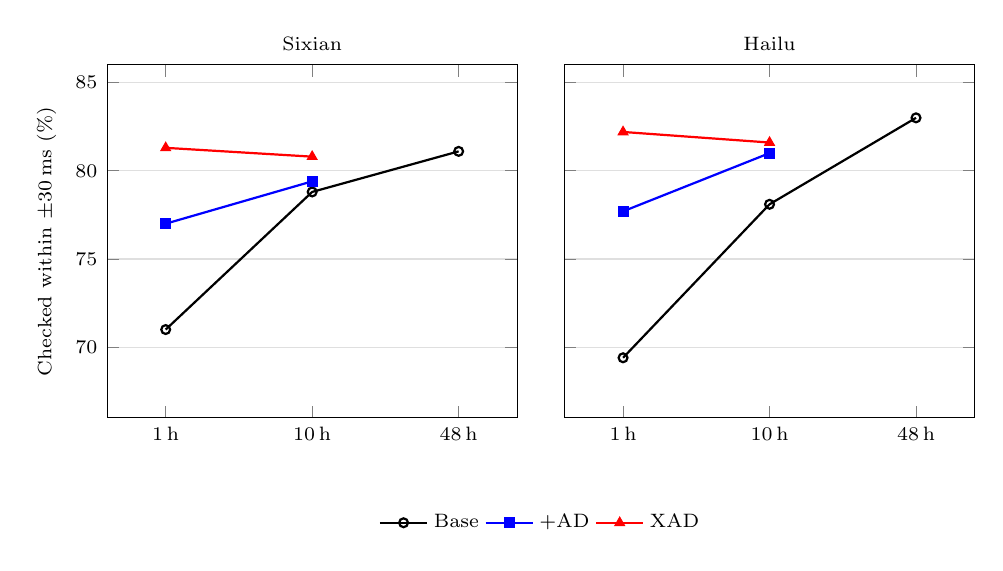
\begin{tikzpicture}
\begin{groupplot}[
  group style={group size=2 by 1, horizontal sep=6mm, y descriptions at=edge left},
  width=0.56\columnwidth, height=0.5\columnwidth,
  symbolic x coords={1\,h,10\,h,48\,h}, xtick=data, enlarge x limits=0.2,
  ymin=66, ymax=86, ytick={70,75,80,85}, ymajorgrids, grid style={gray!25},
  tick label style={font=\scriptsize}, label style={font=\scriptsize}, title style={font=\scriptsize, yshift=-1.5mm},
  legend style={font=\scriptsize, draw=none, fill=none, legend columns=3, at={(1.06,-0.24)}, anchor=north},
  every axis plot/.append style={thick, mark size=1.6pt}]
\nextgroupplot[title=Sixian, ylabel={Checked within $\pm$30\,ms (\%)}]
\addplot[black, mark=o] coordinates {(1\,h,71.0) (10\,h,78.8) (48\,h,81.1)};
\addplot[blue, mark=square*] coordinates {(1\,h,77.0) (10\,h,79.4)};
\addplot[red, mark=triangle*] coordinates {(1\,h,81.3) (10\,h,80.8)};
\legend{Base, +AD, XAD}
\nextgroupplot[title=Hailu]
\addplot[black, mark=o] coordinates {(1\,h,69.4) (10\,h,78.1) (48\,h,83.0)};
\addplot[blue, mark=square*] coordinates {(1\,h,77.7) (10\,h,81.0)};
\addplot[red, mark=triangle*] coordinates {(1\,h,82.2) (10\,h,81.6)};
\end{groupplot}
\end{tikzpicture}
\caption{Checked-syllable timing accuracy versus training data (three seeds at 1 and 10\,h; the rightmost point is a single 48.0/47.2-h Base model). 95\% CIs are about $\pm$4 points.}
\label{fig:size}
\end{figure}

\subsection{ASR check}
Table~\ref{tab:asr} gives an independent view from a recognizer that never saw our aligner or classifier. Overall CER does not separate the 1-h systems ($-$0.5 [$-$2.7, +1.9] points for XAD), while the 48-h baseline is better ($-$2.6 [$-$4.5, $-$0.5]). The differences appear where XAD targets them. Checked syllables keep their stop coda more often (+4.8 [1.6, 8.0] points), the handicap of checked words relative to other words shrinks from $-$4.1 to $-$0.5 points (+3.6 [1.2, 6.0]), and tone marks agree more often with those of natural speech (+3.2 [1.9, 4.4]). The 48-h baseline improves tone marks equally but leaves the checked-word handicap almost unchanged ($-$3.7), which suggests that the checked-syllable gain comes from duration supervision rather than from more data. With +AD alone the same pattern holds with smaller gains (+3.7, +2.6, and +2.8 points). As an upper bound, copy-synthesis (natural mel spectrograms through the same vocoder) reaches 89.4\% retention, a gap of +0.2, and 88.9\% tone agreement. XAD thus removes the checked-word handicap and closes about 40\% of the retention gap between Base and this bound, while the large CER difference (9.8\% vs.\ 21.7\%) shows that most of what remains is general acoustic quality rather than timing.

\begin{table}[t]
\centering
\caption{ASR check (Omnilingual ASR, both varieties pooled, 180 sentences; \%). Gap: letter similarity of checked words minus other words. Copy-synthesis: natural mel spectrograms through the same vocoder (upper bound). CIs of the differences are given in the text.}
\label{tab:asr}
\footnotesize
\setlength{\tabcolsep}{3.5pt}
\begin{tabular}{lcccc}
\toprule
System & CER $\downarrow$ & Checked kept $\uparrow$ & Gap $\uparrow$ & Tone marks $\uparrow$ \\
\midrule
Base          & 22.2 & 77.8 & $-$4.1 & 73.9 \\
+AD           & 21.8 & 81.5 & $-$1.5 & 76.7 \\
XAD           & 21.7 & \textbf{82.6} & \textbf{$-$0.5} & 77.1 \\
Base, 48\,h   & 19.6 & 80.1 & $-$3.7 & 77.2 \\
\midrule
Copy-synthesis & 9.8 & 89.4 & +0.2 & 88.9 \\
\bottomrule
\end{tabular}
\end{table}

\subsection{What did not help}
Inference-time duration scaling, dropout in or pre-training of the duration predictor, replaying source-variety data during target training, and averaging the durations of several seeds gave no further gain over XAD.

\section{Discussion and Limitations}
At one hour, alignment supervision accounts for most of the timing gain (6.0 of 10.3 points for Sixian, 8.3 of 12.8 for Hailu), while cross-variety initialization with the larger predictor contributes most of the spectral gain and about half of the tonal gain. The remaining vowel-duration errors concentrate before pauses, where the predictor lengthens vowels more than the speakers do. % TODO: keep only if you want to report this qualitative finding
The study has limitations. We have not yet completed a listening test, so all results are objective; a paired-comparison listening test is under way. % TODO: update if listening-test results arrive
All systems share one architecture and vocoder. The recipe needs a pronunciation lexicon and an in-domain aligner. The high-resource reference is a single model. The ASR model and the tone classifier are imperfect judges: the classifier reaches only 71.5\% and 67.1\% on natural speech.

\section{Conclusion}
XAD-TTS combines cross-variety initialization with alignment-supervised durations and an enlarged duration predictor. With one hour of Hakka speech, it brings checked-syllable timing to the level of a baseline trained on 48 hours, reduces spectral distortion, and improves objective tone recognition in both Sixian and Hailu, and an independent multilingual recognizer confirms the gains on checked syllables and tones. The recipe adds no inference-time component and trains in about two hours on a single consumer GPU, which makes it a practical starting point for voices in other low-resource varieties.

% TODO: acknowledgment (funding, corpus license)

\bibliographystyle{IEEEtran}
\bibliography{refs}

\end{document}
